\section{Implementation, Integration and Test Plan}
\subsection{Overview}
Questo capitolo tratta l'implementazione del sistema, l'integrazione dei componenti e il piano di test. L'obiettivo dei test è individuare e correggere la maggior parte dei bug prima del rilascio dell'applicazione. Si sottolinea che l'implementazione e l'integrazione sono processi che vanno di pari passo; spesso l'ordine di integrazione segue quello dell'implementazione. Durante la definizione della strategia di implementazione, si considera anche il piano di test di integrazione.

\subsection{Implementation Plan}
Il piano di implementazione e testing del nostro sistema seguirà una strategia combinata bottom-up e thread, al fine di sfruttare i vantaggi di entrambi gli approcci.


\noindent \textbf{Strategia Bottom-Up}
La strategia bottom-up si concentra sull'integrazione incrementale dei componenti del sistema, partendo dalle parti più basilari e procedendo verso le funzionalità più complesse. Questo metodo offre diversi vantaggi:

\begin{enumerate}
    \item Facilità nel Tracking dei Bug: Poiché l'integrazione avviene progressivamente, è più semplice identificare e risolvere i bug nei moduli di base prima che essi influenzino componenti più ampi.
    \item Test Incrementali: Ogni componente può essere testato man mano che viene integrato, permettendo di validare ogni parte del sistema in fasi successive.
    \item Flessibilità e Adattabilità: Questo approccio permette una maggiore flessibilità, poiché le modifiche possono essere apportate più facilmente durante le prime fasi di sviluppo.
\end{enumerate}

\noindent \textbf{Strategia Thread}
La strategia thread, nel nostro contesto, implica l'identificazione e l'implementazione delle funzionalità del sistema tramite diversi thread di esecuzione. I vantaggi includono:

\begin{enumerate}
    \item Consegne Intermedie Valutabili: Attraverso l'uso di thread, si possono produrre deliverable intermedi che possono essere valutati dai stakeholder, facilitando la validazione del sistema realizzato.
    \item Parallelismo nello Sviluppo: Diverse funzionalità possono essere sviluppate in parallelo da diversi team, aumentando l'efficienza e riducendo i tempi di sviluppo.
\end{enumerate}

\subsubsection{Features identification}
Nella fase di "Identificazione delle Funzionalità", elenchiamo e analizziamo le caratteristiche chiave del sistema. Questo processo è fondamentale per comprendere l'ordine di implementazione dei componenti, dato che alcune funzionalità dipendono da altre precedentemente implementate.\\
\noindent \textbf{[F1] Sign in and sign up}\\
 Queste sono le funzionalità base che consentono agli utenti di accedere e utilizzare la piattaforma. Devono essere implementate per prime, in quanto sono il punto di ingresso per studenti ed educatori e sono prerequisiti per tutte le altre funzionalità.\\
\noindent \textbf{[F2] Tournament management}\\
 Dopo aver stabilito l'accesso degli utenti, il passo successivo è consentire agli educatori di creare e gestire tornei. Questa funzionalità è fondamentale perché struttura l'intero contesto in cui si svolgono le battle. Senza la gestione dei tornei, non sarebbe possibile organizzare e coordinare le sfide di programmazione.\\
\noindent \textbf{[F3] Battle management}\\
 Una volta che i tornei sono configurati, è necessario implementare la gestione delle singole battaglie. Questo include l'upload dei code kata, la definizione dei team, e la configurazione delle scadenze. Le battaglie sono l'elemento centrale dell'interazione degli studenti sulla piattaforma e dipendono dalla previa configurazione dei tornei.\\
\noindent \textbf{[F4] Evaluation}\\
Con le battaglie in corso, è fondamentale avere un sistema di valutazione che analizzi le soluzioni inviate dagli studenti. Questo processo include la verifica delle soluzioni rispetto ai test case e la valutazione manuale da parte degli educatori. La funzionalità di valutazione deve seguire la gestione delle battaglie, in quanto è essenziale per determinare i punteggi delle squadre.\\
\noindent \textbf{[F5] Ranking management}\\
Dopo la valutazione delle battaglie, è necessario gestire i ranking sia delle singole battaglie che dei tornei complessivi. Questo permette agli studenti e agli educatori di vedere le prestazioni, creando un contesto competitivo. Questa funzionalità dipende dalla valutazione delle battaglie e dalla gestione dei tornei e delle battaglie.\\
\noindent \textbf{ Notifications management}\\
This is the feature that manages the notifications for the user.
A differenza delle altre funzionalità, la gestione delle notifiche  sarà sviluppata e raffinata continuamente durante l'intero processo di sviluppo. Non seguono un ordine fisso ma sono integrate e adattate in base al progresso delle altre funzionalità.

\subsection{Component Integration and Testing}
Nella sezione successiva, mostreremo per ogni fase quali componenti vengono implementati, come avviene l'integrazione di questi componenti e le modalità di test a cui sono sottoposti, supportati da un diagramma di integrazione specifico per ciascuna fase.\\

The first step is to implement the Model, which is the component that implements all methods that allow access to the Database and perform queries and updates on it. Since we are following a bottom up approach, we will use drivers to test the integration of the components, as it can be seen from the following diagrams:

\begin{figure}[H]
    \centering
    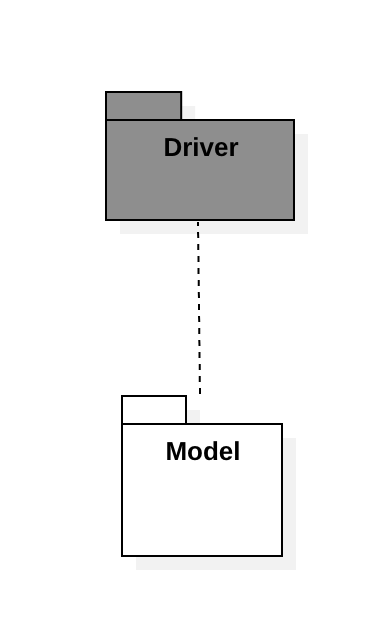
\includegraphics[width=0.3\textwidth]{Test/Model.png}
    \label{fig:enter-label}
\end{figure}

%%%%%%%%%%%%%%%%%%
\textbf{[F1] Sign in and sign up developing}
Subsequently, we focus on building out the authentication mechanism first and part of the User notification component  because the SignUpManager  uses it to send email to users.

\begin{figure}[H]
    \centering
    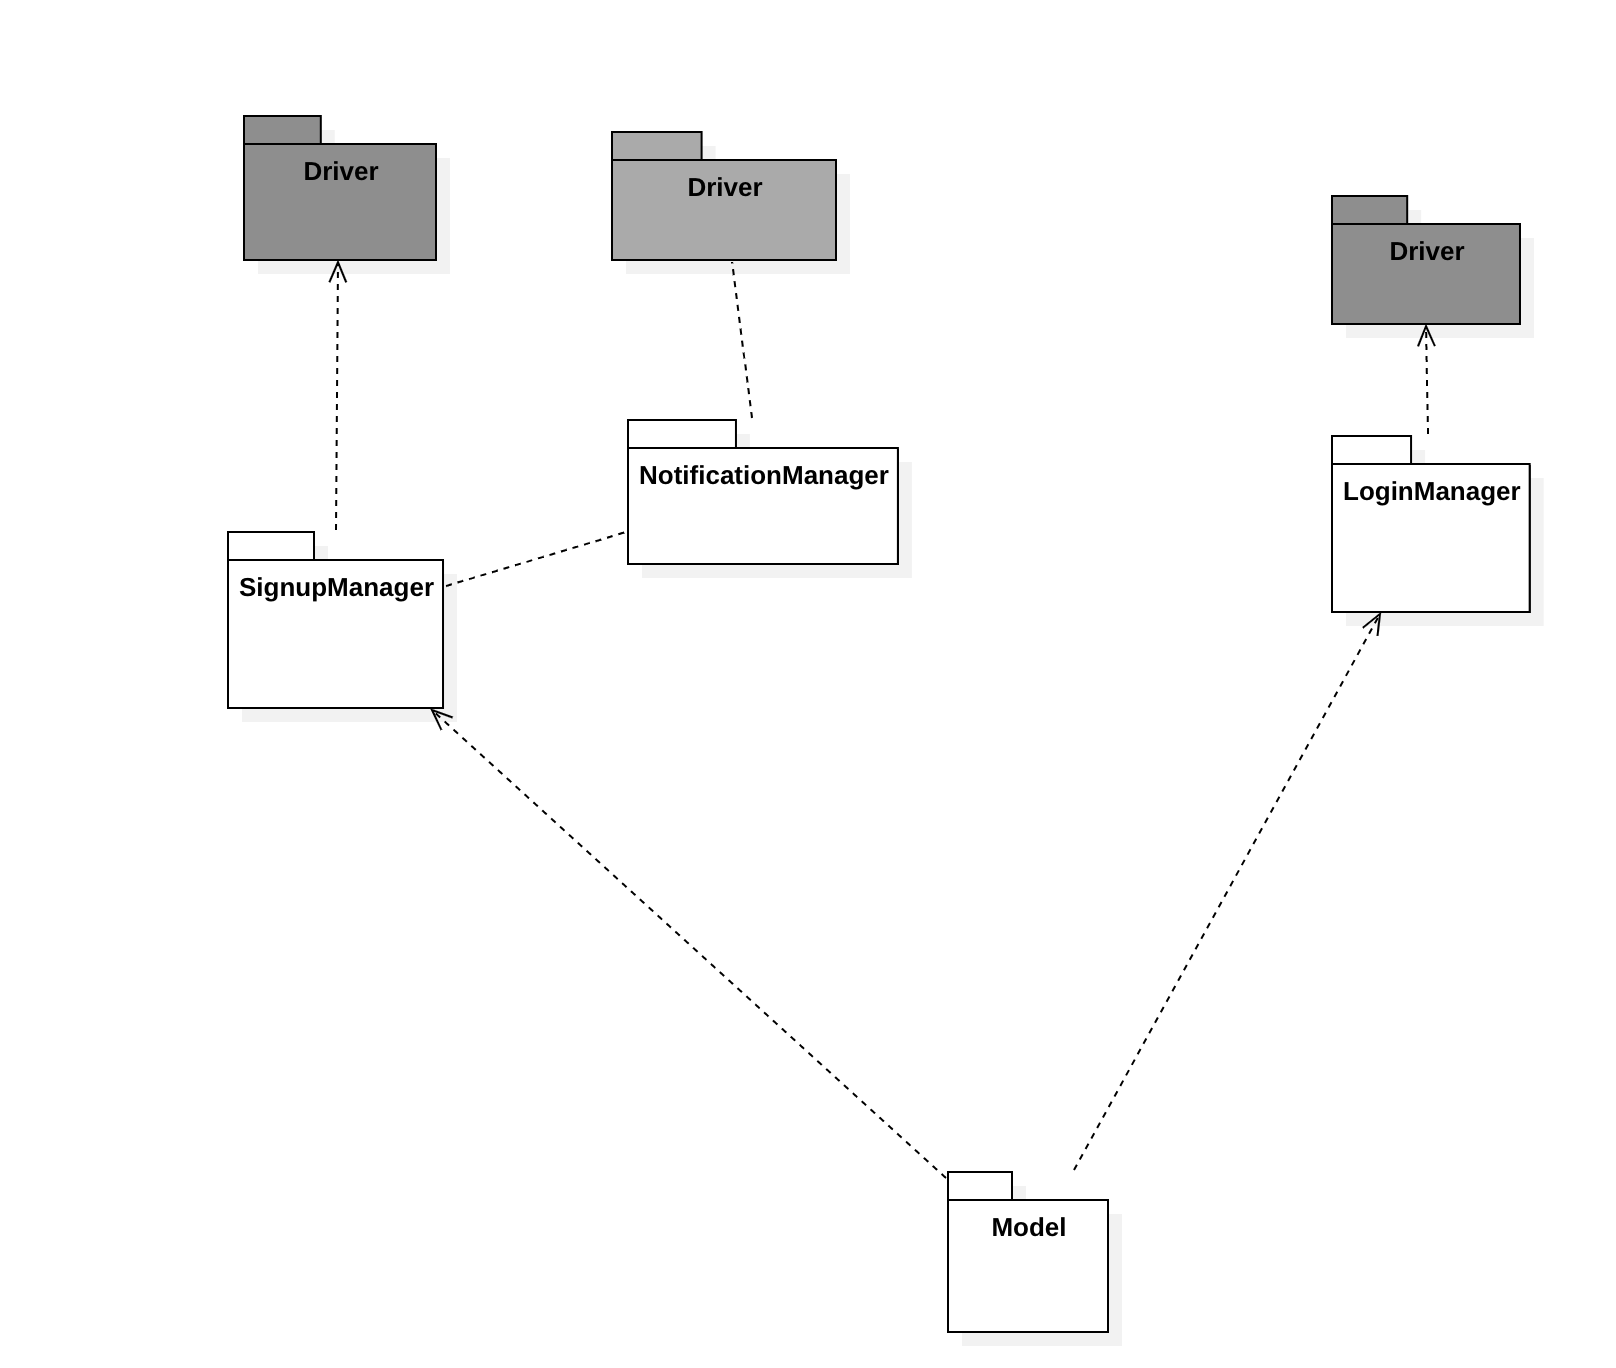
\includegraphics[width=0.56\textwidth]{Test/Login.png}
    \label{fig:enter-label}
\end{figure}
%%%%%%%%%%%%%%%%%
\textbf{[F2] Tournament management}
Following the authentication setup, we turn our attention to the tournament management aspect, since it serves as a foundation for subsequent functionalities that hinge on its proper operation. Alongside this, a segment of the Notification Manager is also implemented. This integration is vital as it plays a key role in tournament management, particularly in notifying subscribed users about tournament creation.
\begin{figure}[H]
    \centering
    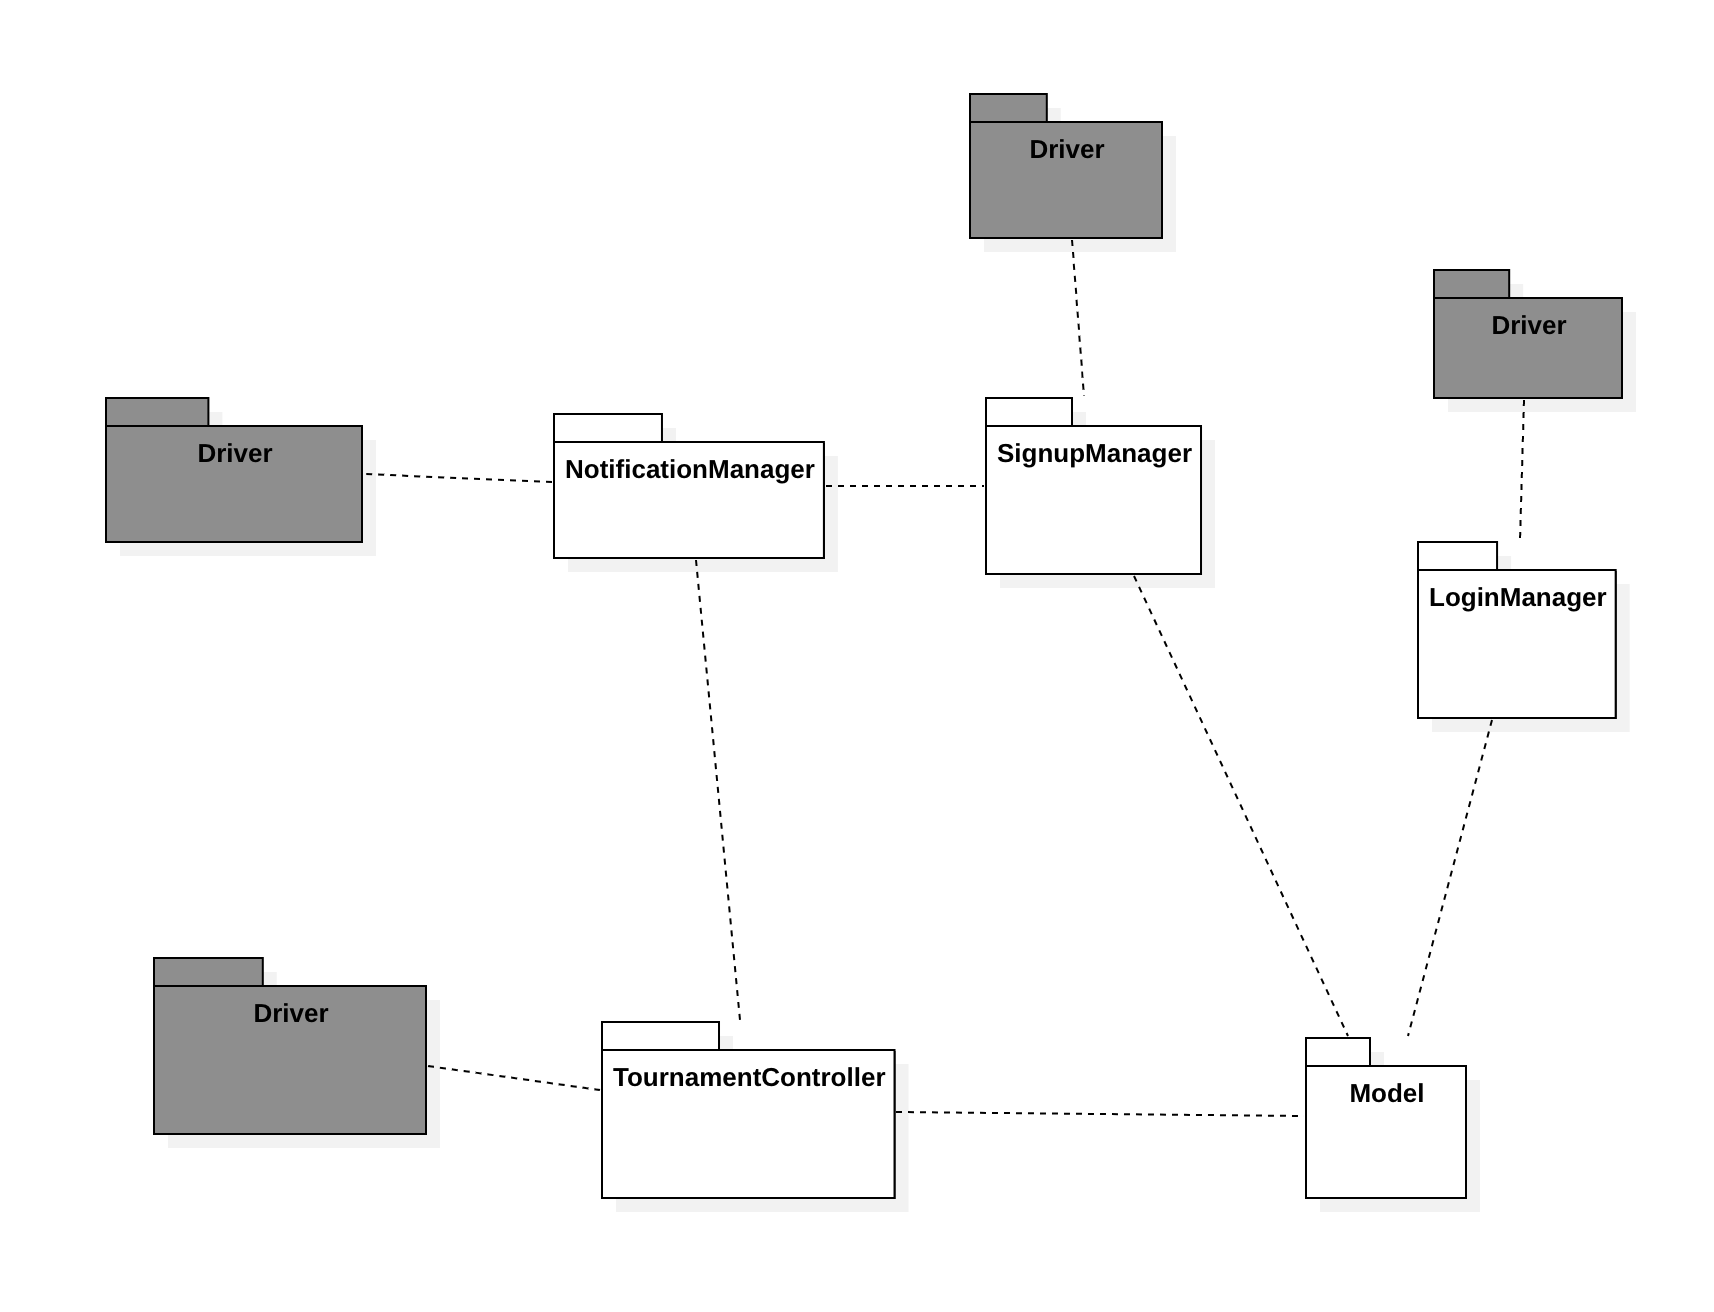
\includegraphics[width=0.56\textwidth]{Test/Tournament.png}
    \label{fig:enter-label}
\end{figure}
%%%%%%%%%%%%%%%%%
\textbf{[F3] Battle management}
Our next focus is on developing the battle management system. 
\begin{figure}[H]
    \centering
    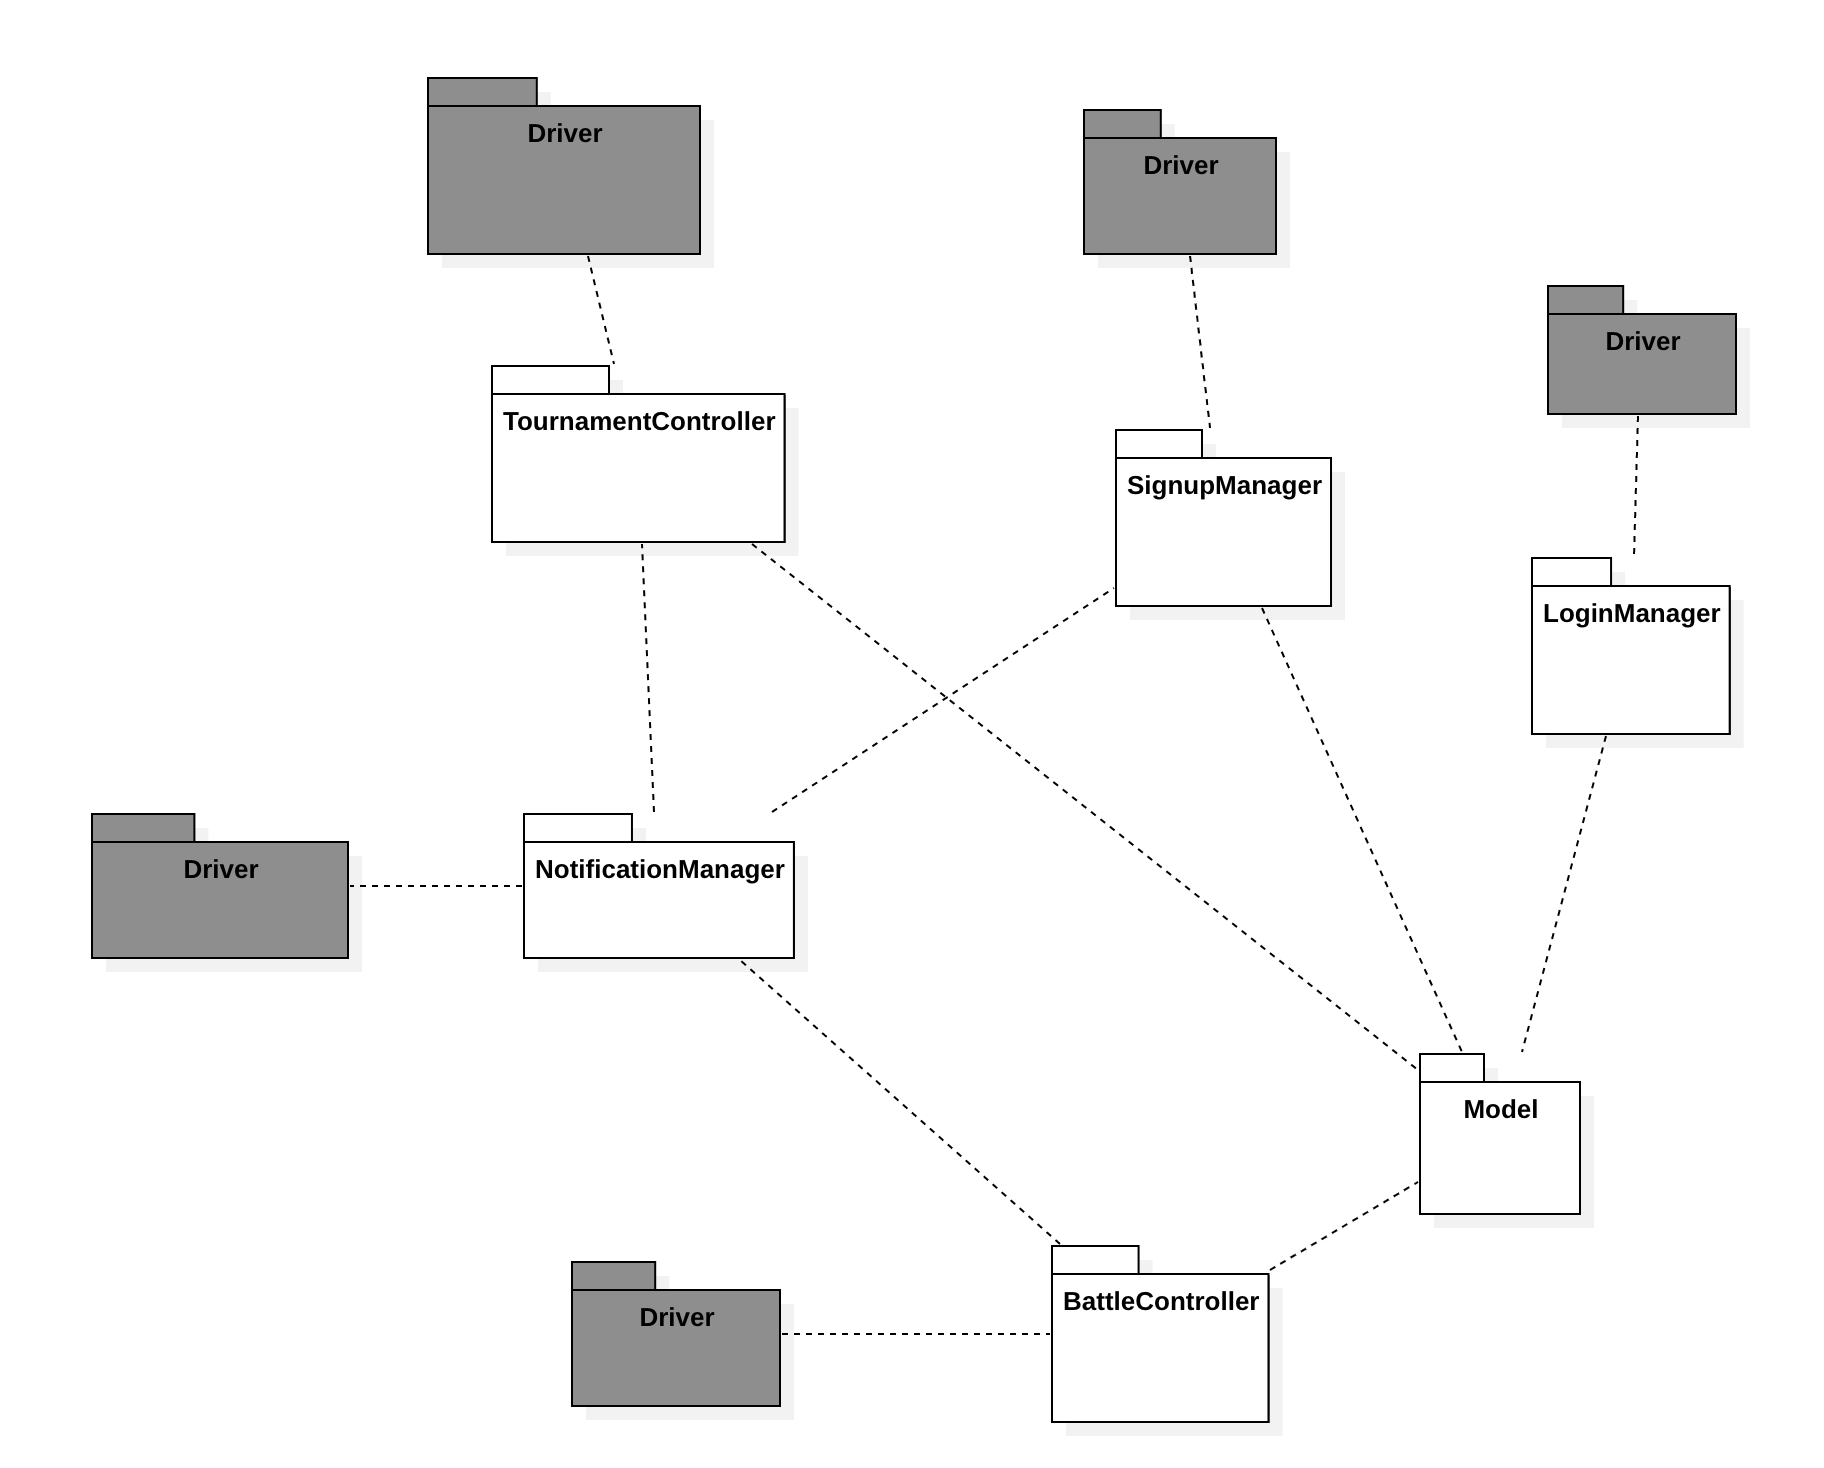
\includegraphics[width=0.56\textwidth]{Test/Battle.png}
    \label{fig:enter-label}
\end{figure}
%%%%%%%%%%%%%%%%%
\textbf{[F4] Evaluation}
After the battle management component is fully operational, we advance to the development of the evaluation system. This component encompasses both automated and manual assessment methods, designed to evaluate the outcomes of the battles. The placement of the evaluation system in the development sequence is strategic, as it relies heavily on data generated from completed battles. Alongside this, a segment of the Notification Manager is also implemented. This integration is vital as it plays an important role in battle management.
\begin{figure}[H]
    \centering
    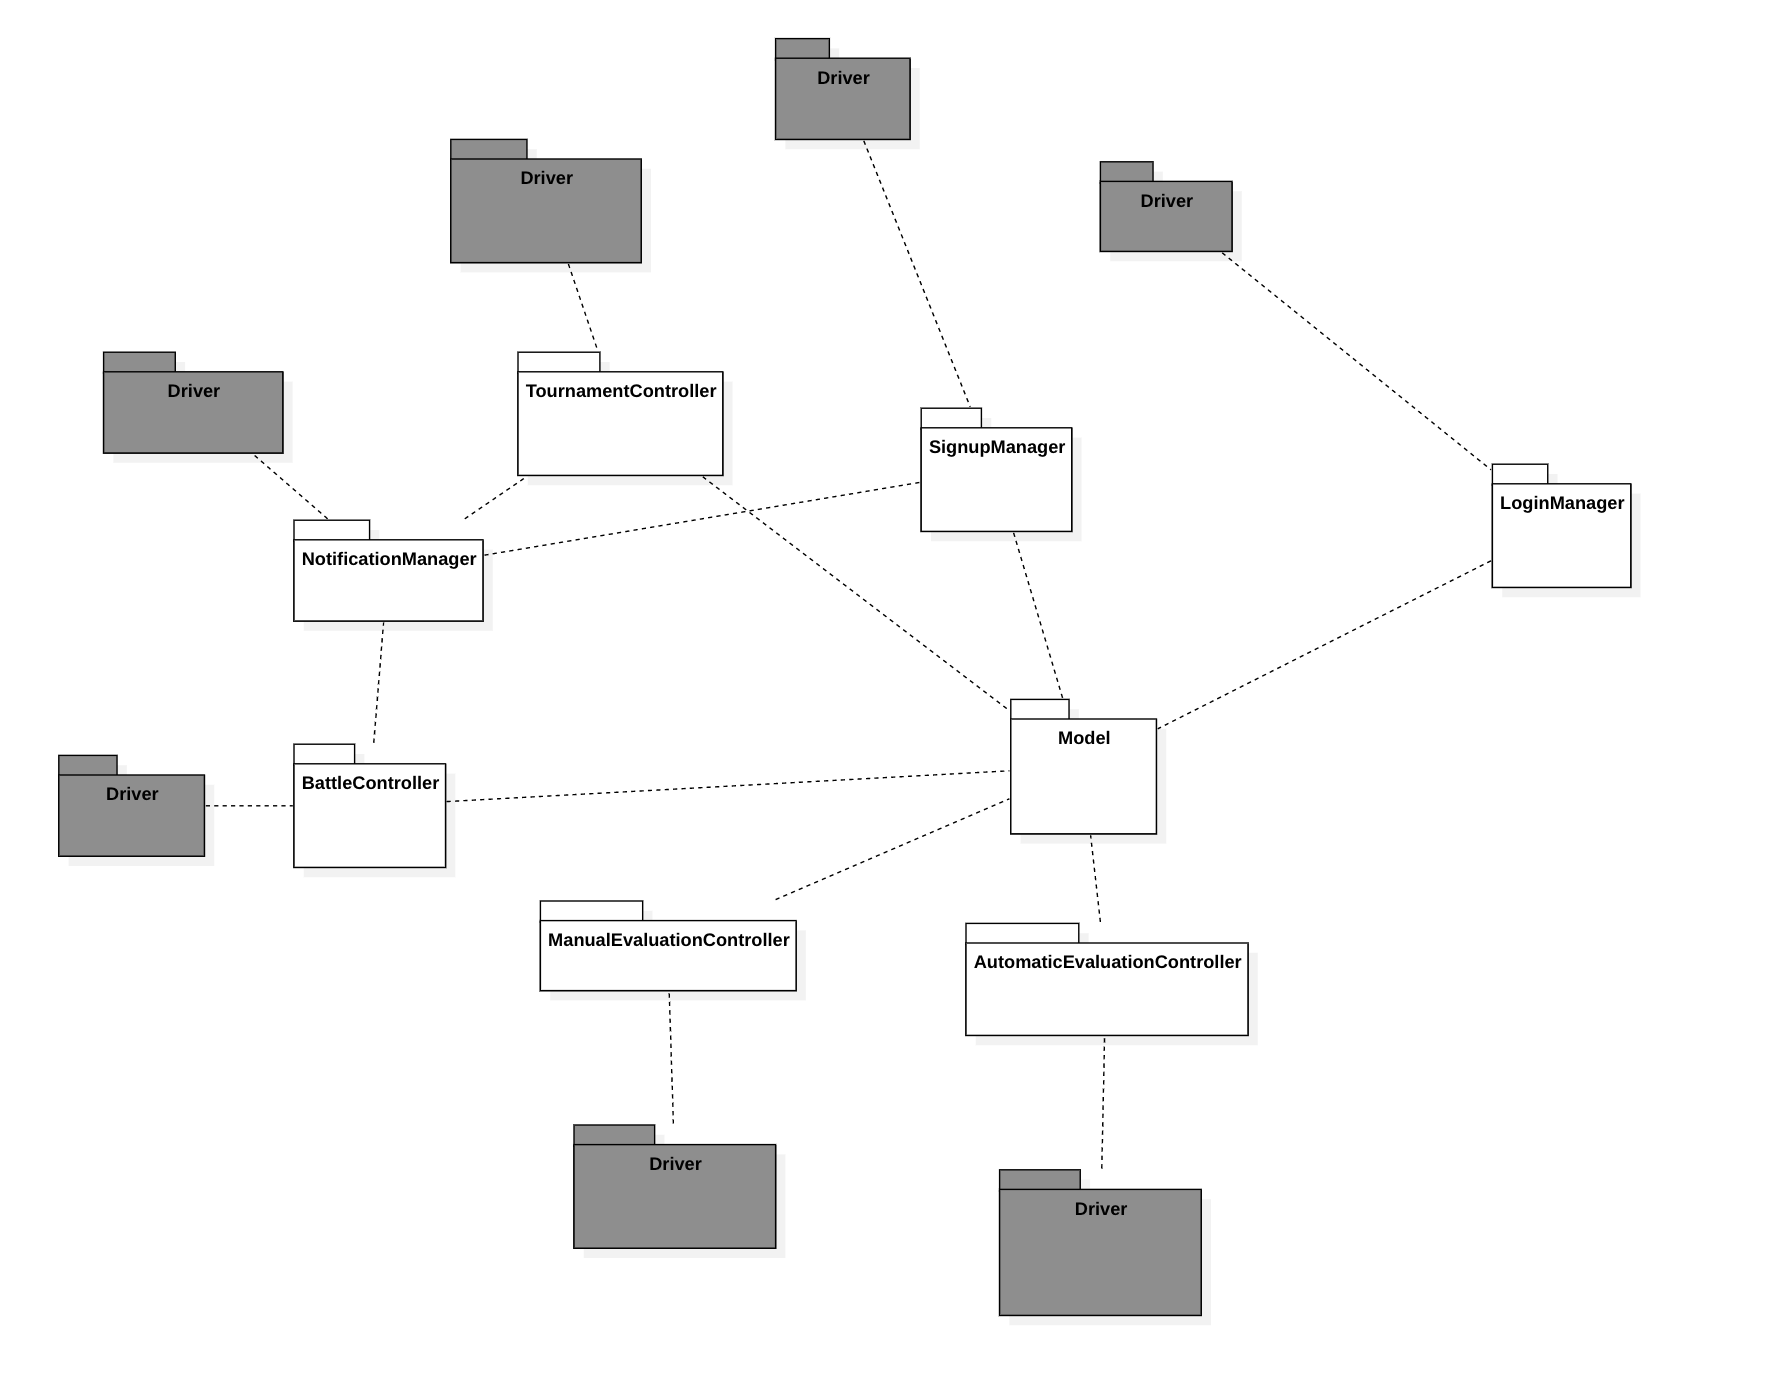
\includegraphics[width=0.56\textwidth]{Test/Evaluation.png}
    \label{fig:enter-label}
\end{figure}
%%%%%%%%%%%%%%%%%
\textbf{[F5] Ranking management}
Following the evaluation system, our attention shifts to the development of the ranking component. This feature is essential as it compiles and displays the results of the battles and tournaments, providing a clear and concise representation of participants' standings.
\begin{figure}[H]
    \centering
    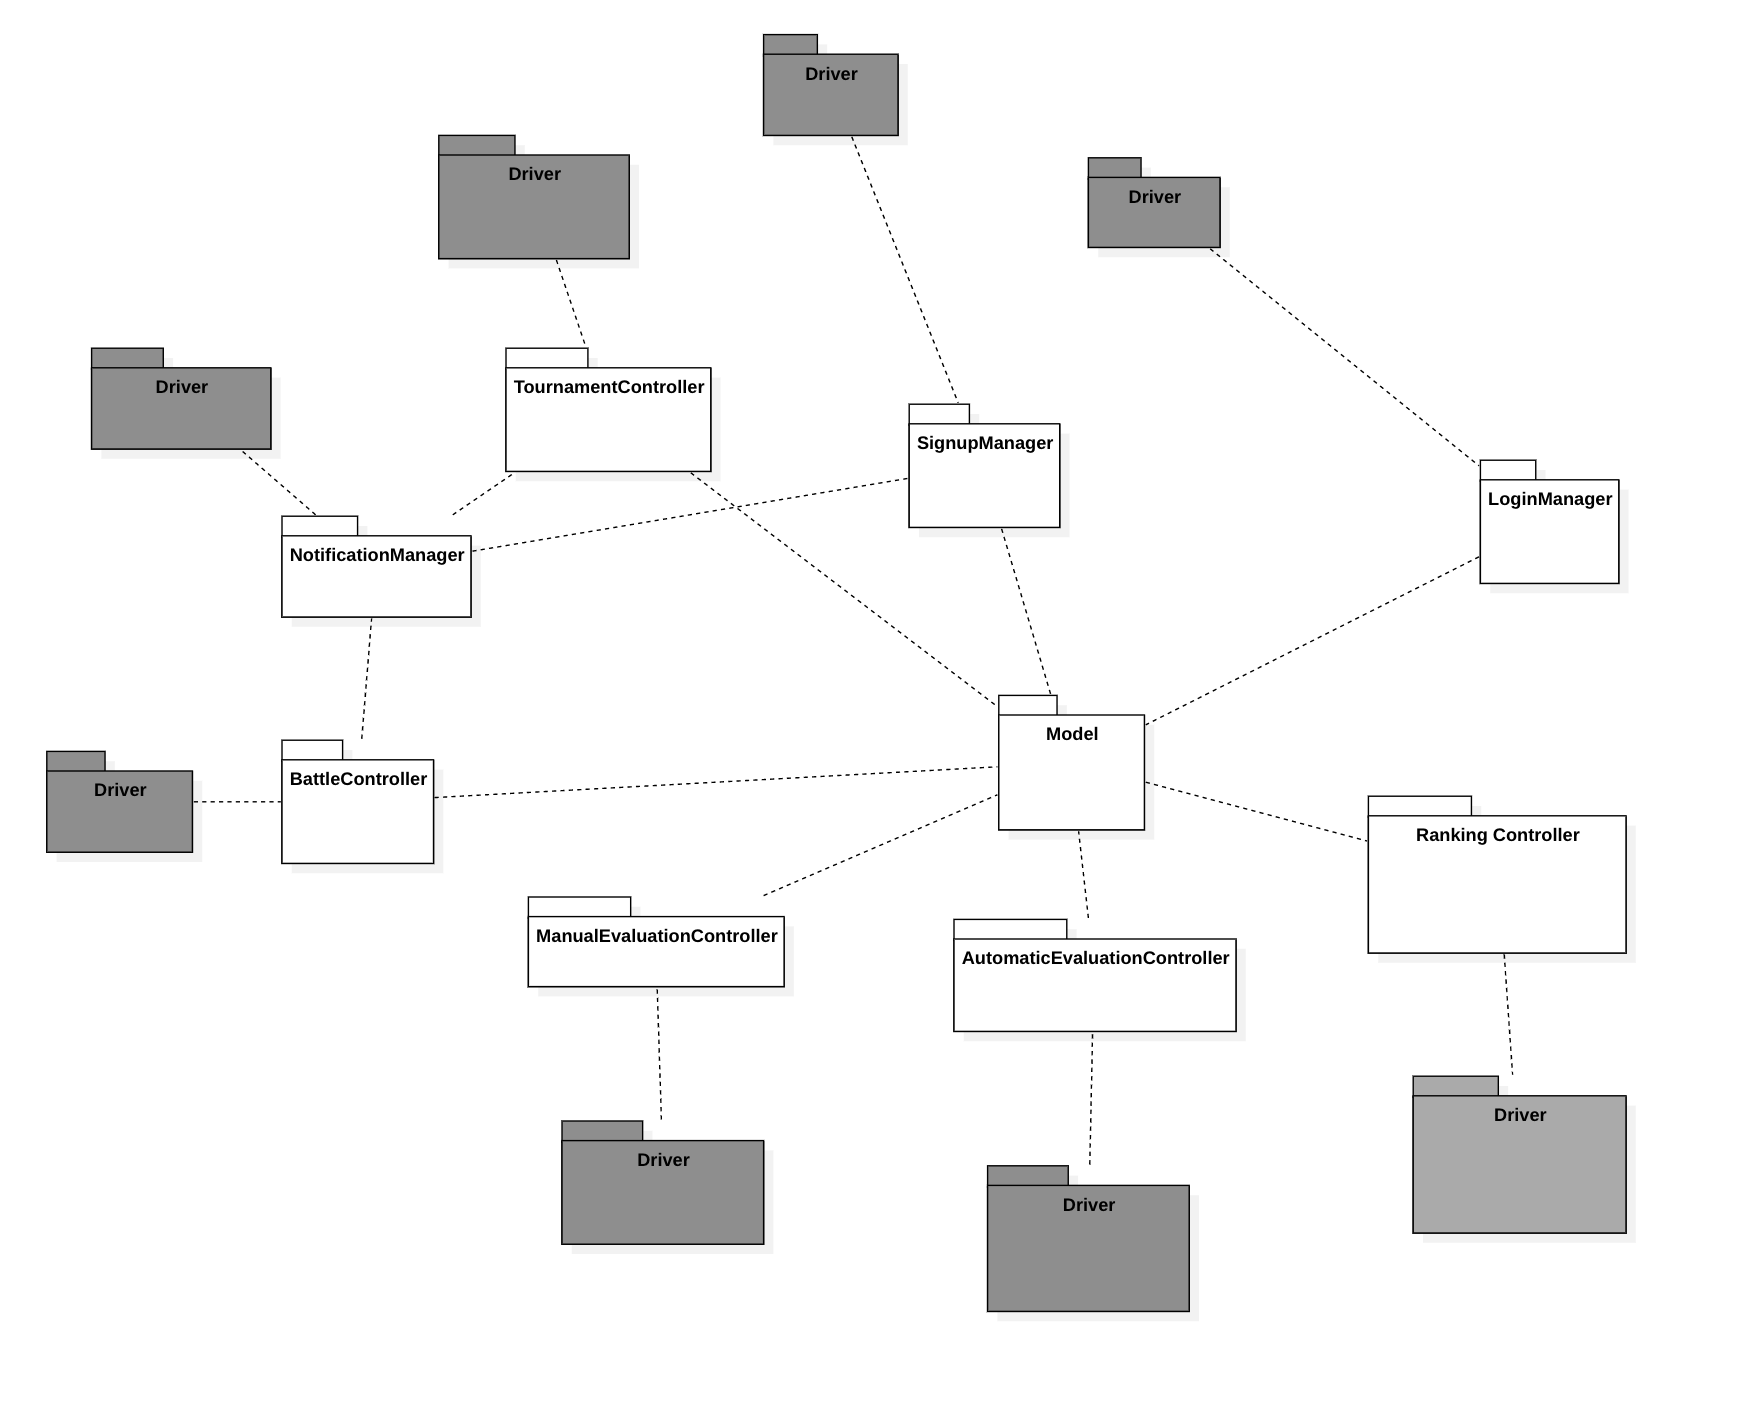
\includegraphics[width=0.56\textwidth]{Test/Ranking.png}
    \label{fig:enter-label}
\end{figure}
%%%%%%%%%%%%%%%%%
\subsection{System testing}
Dopo l'integrazione dei componenti nel sistema CKB, procediamo  con una serie di test. L'obiettivo è garantire che le funzionalità rispondano alle aspettative e che l'applicazione si comporti adeguatamente sotto diversi carichi di lavoro. Si delineano quindi vari ambiti di test, ognuno focalizzato su specifiche esigenze:

\begin{itemize}

 \item \textbf{Functional Testing}: Per verificare  che ogni singola funzione della piattaforma, dalle notifiche agli aggiornamenti dei punteggi, operi correttamente secondo le specifiche. 

  
  \item \textbf{Performance Testing}:Valuta la velocità, la reattività e la stabilità dell'applicazione sotto vari carichi di lavoro. E' importante per assicurare che le performance dell'applicazione siano all'altezza delle sfide, specialmente quando la piattaforma calcola in tempo reale i punteggi delle competizioni, elemento centrale dell'esperienza utente su CKB.
  
  \item \textbf{Load Testing}:Verifica la capacità dell'app di gestire un volume elevato di utenti o transazioni simultaneamente.
  
  \item \textbf{Stress Testing}: Per spingere il sistema oltre i limiti operativi abituali e osservare la sua capacità di mantenere l'integrità e la sicurezza delle operazioni anche in condizioni estreme.
  
\end{itemize}
All the tests in general are fundamental for studying the behavior of the system.



\subsection{Acceptance Testing}

Successivamente ai test descritti in precedenza, procederemo con il testing di accettazione da parte dell'utente. Questo passaggio è cruciale: anche se abbiamo verificato il rispetto dei requisiti funzionali e non-funzionali, resta indispensabile ottenere il benestare finale da parte del committente.

Il testing di accettazione si svolge seguendo un approccio black-box, che coinvolge gli utenti in interazioni con il sistema che riflettono l'utilizzo reale. Questo metodo consente di confermare se il software soddisfa le specifiche desiderate in origine dal cliente. È un controllo definitivo che valida la piena corrispondenza del prodotto alle aspettative e alle necessità per cui è stato commissionato.





